\begin{figure}[t!]
    \centering
    \begin{subfigure}[b]{\textwidth}
        \centering
        % \begin{tikzpicture}[
        %     scale=1, auto, node distance=2cm, 
        %     every edge/.style={draw, <-, font=\small},
        %     state/.style={circle, fill=mylightgrey, draw=black, text=black}
        % ]
        %     % Nodes
        %     \node[state] (s1) at (0,0) {$s$};
        %     % Edges
        %     \path[->]
        %         (s1) edge[out=160, in=200, loop, looseness=8, draw=black] node[pos=0.5, left, text=black] {\textcolor{mygrey}{$\best{\pi}(s) :=$} 1} (s1)
        %         (s1) edge[out=20, in=340, loop, looseness=8, draw=black] node[pos=0.5, right, text=black] {0 \textcolor{mygrey}{$=: \worst{\pi}(s)$}} (s1) ;
        %         % (s1) edge[out=145, in=215, loop, looseness=7] 
        %         %     node[pos=0.5, right] {$\best{a}$} 
        %         %     node[pos=0.5, left] {1} 
        %         % (s1)
        %         % (s1) edge[out=35, in=325, loop, looseness=7] 
        %         %     node[pos=0.5, left] {$\worst{a}$} 
        %         %     node[pos=0.5, right] {0} 
        %         % (s1);
        % \end{tikzpicture}
        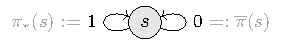
\includegraphics[width=0.35\linewidth]{figures/mdp.pdf}
        \caption{MDP}
        \label{fig: experiment smallest MDP for iv vs fv}
    \end{subfigure}%
    \\
    \vspace{0.5cm}
    % --- Subfigure 1: Streamlines ---
    \begin{subfigure}[b]{0.48\textwidth}
        % \begin{tikzpicture}
        %     \begin{axis}[
        %         width=\linewidth,
        %         % title={Initial-visit solutions},
        %         xlabel={$q(s, \pi_*(s))$},
        %         ylabel={$q(s, \overline \pi(s))$},
        %         tick label style={font=\small},
        %         label style={font=\small},
        %         xmin=0, xmax=5,
        %         ymin=-0.5, ymax=4.5,
        %         % grid=off,
        %         axis equal image,
        %         unbounded coords=jump, % This handles the NaN values in your CSV
        %         xtick={1, 2,4},
        %         % xticklabels={1, $\frac{1}{1-\gamma}$, 4},
        %         ytick={0, 1,4}
        %     ]

        %         \addplot [black, thin, dotted, domain=-0.5:5, samples=2] {x};
                
        %         % 1. Plot the streamlines from CSV
        %         \addplot[mygrey, thin, forget plot] table [col sep=comma, x index=0, y index=1] {figures/streamlines-iv.csv};

        %         % 2. Plot the simulation trajectory
        %         \addplot[CambridgeCoreBlue, thick] table [col sep=comma, x index=0, y index=1] {figures/simulation-iv-above.csv};

        %         \addplot[CambridgeCoreBlue, thick] table [col sep=comma, x index=0, y index=1] {figures/simulation-iv-below.csv};
                
        %         % 3. Mark Attractors (x1 and x2 based on your gamma=0.5)
        %         \node[label={right:$q_{\pi_*}$}, circle, fill, inner sep=1.5pt] at (axis cs:2, 1) {};
                
        %         \node[label={right:$q_{\overline \pi}$}, circle, fill, inner sep=1.5pt] at (axis cs:1,0) {};
                
        %         % 4. Start Points with Labels
        %         % Point A: Using your x0 = [3.75, 4]
        %         \node[label={left:$q$}, circle, fill, inner sep=1.5pt, CambridgeCoreBlue] at (axis cs:3.75, 4) {};
                
        %         % Point B: Placeholder (Update coordinates as needed)
        %         \node[label={below:$q'$}, circle, fill, inner sep=1.5pt, CambridgeCoreBlue] at (axis cs:4, 3.75) {};
        %     \end{axis}
        % \end{tikzpicture}
        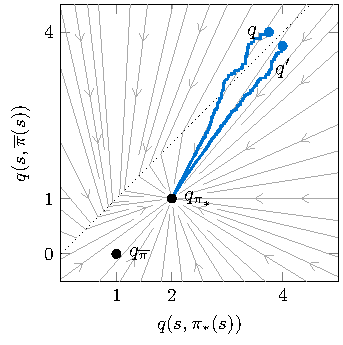
\includegraphics[width=0.8\linewidth]{figures/iv-sol.pdf}
        \caption{Initial-visit solutions}
        \label{fig: iv versus fv simulations IV}
    \end{subfigure}
    \hfill
    % --- Subfigure 2: Placeholder or Second Simulation ---
    \begin{subfigure}[b]{0.48\textwidth}
        % \begin{tikzpicture}
        %     \begin{axis}[
        %         width=\linewidth,
        %         % title={First-visit solutions},
        %         xlabel={$q(s, \pi_*(s))$},
        %         ylabel={$q(s, \overline \pi(s))$},
        %         tick label style={font=\small},
        %         label style={font=\small},
        %         xmin=0, xmax=5,
        %         ymin=-0.5, ymax=4.5,
        %         % grid=off,
        %         axis equal image,
        %         unbounded coords=jump, % This handles the NaN values in your CSV
        %         xtick={1, 2,4},
        %         % xticklabels={1, $\frac{1}{1-\gamma}$, 4},
        %         ytick={0, 1,4}
        %     ]

        %         \addplot [black, thin, dotted, domain=-0.5:5, samples=2] {x};
                
        %         % 1. Plot the streamlines from CSV
        %         \addplot[mygrey, thin, forget plot] table [col sep=comma, x index=0, y index=1] {figures/streamlines-fv.csv};

        %         % 2. Plot the simulation trajectory
        %         \addplot[CambridgeCoreBlue, thick] table [col sep=comma, x index=0, y index=1] {figures/simulation-fv-above.csv};

        %         \addplot[CambridgeCoreBlue, thick] table [col sep=comma, x index=0, y index=1] {figures/simulation-fv-below.csv};
                
        %         % 3. Mark Attractors (x1 and x2 based on your gamma=0.5)
        %         \node[label={right:$q_{\pi_*}$}, circle, fill, inner sep=1.5pt] at (axis cs:2, 1) {};
                
        %         \node[label={right:$q_{\overline \pi}$}, circle, fill, inner sep=1.5pt] at (axis cs:1,0) {};
                
        %         % 4. Start Points with Labels
        %         % Point A: Using your x0 = [3.75, 4]
        %         \node[label={left:$q$}, circle, fill, inner sep=1.5pt, CambridgeCoreBlue] at (axis cs:3.75, 4) {};
                
        %         % Point B: Placeholder (Update coordinates as needed)
        %         \node[label={below:$q'$}, circle, fill, inner sep=1.5pt, CambridgeCoreBlue] at (axis cs:4, 3.75) {};
        %     \end{axis}
        % \end{tikzpicture}
        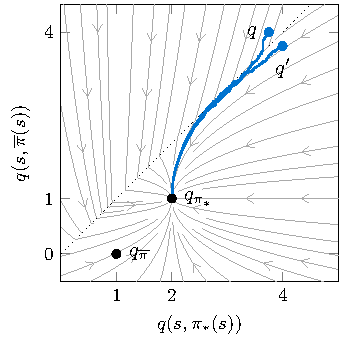
\includegraphics[width=0.8\linewidth]{figures/fv-sol.pdf}
        \caption{First-visit solutions}
        \label{fig: iv versus fv simulations FV}
    \end{subfigure}
    \caption{By avoiding sliding modes, initial-visit solutions sometimes converge to the optimal policy $\best{\pi}$ faster than first-visit solutions despite fewer updates and smaller effective learning rates. The blue lines are MC-O-PI solutions starting in $q$ or $q'$, whereas the grey lines indicate the mean-field flow.}
    \label{fig: iv versus fv simulations}
\end{figure}
